\documentclass[crop,border=7pt]{standalone}
\usepackage{tikz}
\usetikzlibrary{calc,patterns}
\begin{document}
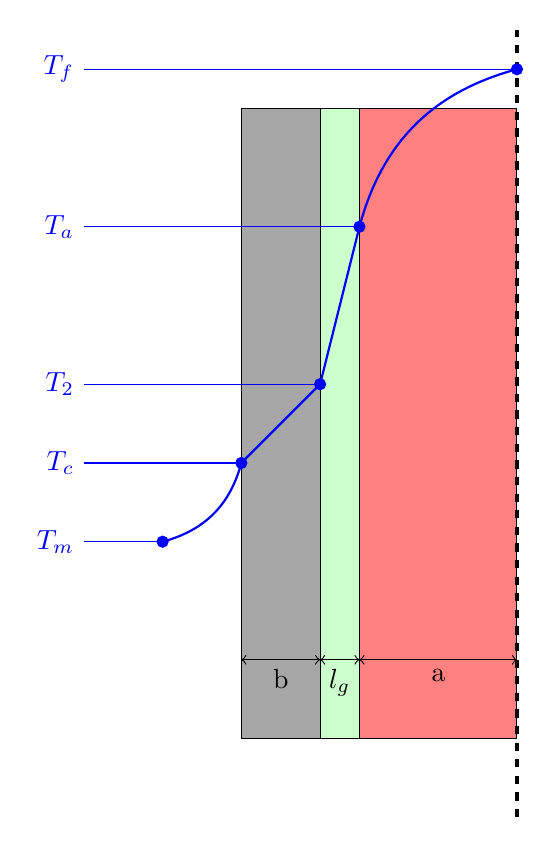
\begin{tikzpicture}

%PROFILE REACTOR
\filldraw[fill=red!50, draw=black] (0,0) rectangle (2,8);
\filldraw[fill=green!20, draw=black] (0,0) rectangle (-0.5,8);
\filldraw[fill=gray!70, draw=black] (-.5,0) rectangle (-1.5,8);
\draw[black, ultra thick, dashed] (2,-1) -- (2,9);


\filldraw[blue] (2,8.5) circle (2pt);
\draw[blue] (2,8.5) -- (-3.5,8.5) node[anchor=east] {$T_f$};
\filldraw[blue] (0,6.5) circle (2pt);
\draw[blue] (0,6.5) -- (-3.5,6.5) node[anchor=east] {$T_a$};
\filldraw[blue] (-.5,4.5) circle (2pt);
\draw[blue] (-.5,4.5) -- (-3.5,4.5) node[anchor=east] {$T_2$};
\filldraw[blue] (-1.5,3.5) circle (2pt);
\draw[blue] (-1.5,3.5) -- (-3.5,3.5) node[anchor=east] {$T_c$};
\filldraw[blue] (-2.5,2.5) circle (2pt);
\draw[blue] (-2.5,2.5) -- (-3.5,2.5) node[anchor=east] {$T_m$};

\draw[blue, thick] (2,8.5) to[bend right] (0,6.5);
\draw[blue, thick] (0,6.5) -- (-.5,4.5);
\draw[blue, thick] (-.5,4.5) -- (-1.5,3.5);
\draw[blue,thick] (-1.5,3.5) to[bend left] (-2.5,2.5);

\draw[black, <->] (2,1)-- (0,1);
\draw[black] (1,1) node[anchor=north] {a};
\draw[black, <->] (0,1) -- (-0.5,1);
\draw[black] (-.25,1) node[anchor=north] {$l_g$};
\draw[black, <->] (-0.5,1) -- (-1.5,1);
\draw[black] (-1,1) node[anchor=north] {b};


 
% \draw[pattern=north east lines,pattern color=violet] (3,0) rectangle (4,35);
% 
% \draw[pattern=north east lines,pattern color=green] (8,0) rectangle (9,35);

% 
% %%LEGEND
% \draw (16.5,30) rectangle (22,35);
% \matrix [below left] at (current bounding box.north east) {
%   \node [yellownode, label=right:\LARGE Inner MOX Fuel] {}; \\
%   \node [rednode, label=right:\LARGE Outer MOX Fuel ] {}; \\
%   \node [bluenode, label=right:\LARGE In-Pile Section] {}; \\
%   \node [blacknode, label=right:\LARGE Plenum Lead] {}; \\
%   
%   \node [graynode, label=right:\LARGE Dummy Section] {}; \\
%   
%   \node [violetnode, label=right:\LARGE Safety Rod] {}; \\
%   
%   \node [greennode, label=right:\LARGE Control Rod] {}; \\
% };


%\draw (0,0) -- (4,0);

%\shade[top color=yellow, bottom color=black] (0,0) rectangle (2,-1);
 %   \filldraw[fill=green!20!white, draw=green!40!black] (0,0) rectangle (2,1);
 %   \draw[pattern=north east lines,pattern color=red] (0,0) rectangle (1,3);
 %   \draw[pattern=north west lines,pattern color=blue] (0,0) rectangle (3,1);
%    \draw[pattern=vertical lines] (2,0) rectangle (5,1);
%    \draw[pattern=horizontal lines,pattern color=yellow] (2,0) rectangle (3,3);

\end{tikzpicture}
\end{document}